\phantomsection
\chapter{Face detection with Viola-Jones}
\label{chap:implementation_violajones}

\noindent The face detection part for this Facial Expression Recognition system is based on Viola-Jones face detection algorithm. This chapter describes how this Viola-Jones algorithm is used and implemented.
\newline

\phantomsection
\section{Viola-Jones}

\vspace{\baselineskip}
\noindent To perform Viola-Jones face detection, video sequences of face are obtained thanks to a webcam or to the Kinect. The algorithm is then able to detect face and regions of interest (ROI) in the frames. The regions of interest are the nose, the left eye, the right eye and the mouth. 
\newline

\noindent Classifiers are trained prior to be used. They are then loaded with a model; one for the face and one for each region of interest. Then, based on these classifiers, face and regions of interest are detected in the frames. Figure~\ref{violajones_implementation_example} shows an example of face detection,along with some regions of interest. In this case of ROI detection, different classifiers have been used for each eye. 
\newline

\begin{figure}[!h]
\begin{center}
\noindent 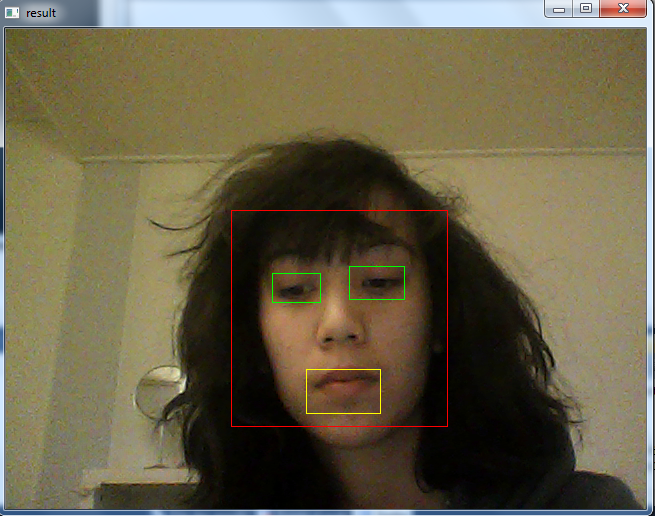
\includegraphics[scale=0.4]{figures/violajones_implementation_example} 
\newline
\caption{Example of face and ROI detection with Viola-Jones}
\label{violajones_implementation_example}
\end{center} 
\end{figure}